\subsection*{Оптическая глубина}


Интенсивность слабого одиночного луча, проходящего через ячейку описывается законом Бэра:
\begin{equation*}
    d I / d x = - \alpha I,
    \hspace{10 mm} 
    \alpha = \alpha (\nu).
\end{equation*}
В хорошем приближение\footnote{
    Для слабого луча [1].
}  $\alpha \neq \alpha(x)$ . 
Введем оптическую длину $\tau(\nu) = l \alpha(\nu)$, тогда
\begin{equation*}
    \sub{I}{out} = \sub{I}{in} e^{- \alpha(\nu) l} = \sub{I}{in} e^{- \tau(\nu)}.
\end{equation*}
Вклад от группы атомов $(v,\, v + d v)$ в $\tau(\nu)$ можем быть записан, как
\begin{equation*}
    d \alpha (\nu, v) = \sigma(\nu, v) \, dn(v),
    \hspace{0.5cm} \Rightarrow \hspace{0.5cm}    
    d \tau(\nu, v) = l \sigma(\nu, v) \, dn(v).
\end{equation*}
Коэффициент поглощения $\sigma(\nu, v)$ имеет Лоренцовский профиль с натуральной шириной $\Gamma$ (?) и смещенной по Допплеру резонансной частотой
\begin{equation}
    \label{1_4}
    \sigma(\nu, v) = \sigma_0 \frac{\Gamma^2/4}{(\nu - \nu_0(1 - v / c))^2 + \Gamma^2/4},
\end{equation}
где $\sigma_0$ -- резонансное сечение поглощения\footnote{
    [1], problem 1: $\sigma_0 \sim n$ атомов в ячейке.
} , зависящее от вида дипольного перехода и поляризации падающего света [1$\Rightarrow$4]. 

Часть атомов $d n (v)$ с определенной скорости можем найти из распределения Больцмана
\begin{equation*}
    d n(v) = n_0 \sqrt{\frac{m}{2 \pi \sub{k}{B} T}} \exp\left(
        - \frac{m v^2}{2 \sub{k}{B} T} 
    \right) \d v,
\end{equation*} 
где $n_0 = N/V$ -- концентрация атомов в ячейке. 

Собирая все вместе (?) приходим к выражению
\begin{equation}
    \label{1_6}
    d \tau (\nu, v) = \frac{2}{\pi} \frac{\tau_0}{\sigma_0 \Gamma} \frac{\nu_0}{c} 
     \sigma(\nu, v) \exp\left(
        - \frac{m v^2}{2 \sub{k}{B} T}
     \right) \d v,
\end{equation}
где $\tau_0$  -- сответствующая нормировка такая, что для резонанса $\tau_0 = \int_v \d \tau (\nu_0,\, v)$.



Для насышенной спектроскопии нужно учесть эффект от дополнительного насыщающего лазерного луча. Из-за него значительная часть атомов в ячейке будут в возбужденном состоянии. Так как атомы могут поглощать свет только когда они в невозможденном состоянии, к \eqref{1_6} добаваить фактор $(\ng-\ne)/N$, описывающей разницу 
между количеством атомов в возбужденном состоянии $\ne$ и невозбужденном $\ng$. 



\subsection*{Скоростные уравнения}


 Населенность в двух состояния описывается скоростными уранениями
\begin{align*}
    \dot{\ng} = \phantom{-}\Gamma N_e - \sigma \Phi (\ng - \ne), \\
    \dot{\ne} = - \Gamma \ne + \sigma \Phi (\ng - \ne),
\end{align*}
где первое слагаемое отвечает спонтанной эмиссии, и второе насыщению лазером. $\Phi = I / h \nu$ -- насыщающий поток фотонов. Учитывая, что $\ng + \ne = N = \const $, можем получить диффур первого порядка на $\ne$:
\begin{equation*}
    \dot{\ne} = - (\Gamma \ne + 2 \sigma \Phi) \ne + \sigma \Phi N.
\end{equation*}
Решение можем быть найдено в виде
\begin{equation*}
    \ne (t) = \left[
        \Gamma \ne(0) - \frac{N \sigma \Phi}{\Gamma + 2 \sigma \Phi} 
    \right] e^{-(\Gamma + 2 \sigma \Phi) t} + \frac{N \sigma \Phi}{\Gamma + 2 \sigma \Phi}.
\end{equation*}

Заметим, что при $\Phi = 0$:
\begin{equation*}
    \ne (t) = \ne (0) e^{- \Gamma t},
\end{equation*}
а в случае слаюого насыщающего луча $\sigma \Phi \ll \Gamma$, и изначальной популяции в невозбужденном состоянии,
\begin{equation*}
    \ne (t) = \frac{N \sigma \Phi}{\Gamma} \left(1 - e^{- \Gamma t}\right),
\end{equation*}
достигающий стационарного состояния после $\Gamma^{-1}$ с $\ne = N \sigma \Phi / \Gamma \ll N$.   Наконец, при $\sigma \Phi \gg \Gamma$, получаем насыщенный переход
\begin{equation*}
    \ne (t) = \left[\ne(0) - N/2\right]e^{-2 \sigma \Phi t} + N / 2 \to N/2.
\end{equation*}
Под насыщением понимаем, что $\ne = N/2$, большие значения по понятным причинам невозможны $\forall  \Phi$, по крайней мере для двухуровневых систем. 

Также наблюдается увеличение <<мощности>> ширины линии перехода, в пределе $(\Gamma + 2 \sigma \Phi) t \gg 1$, получаем
\begin{equation*}
     \frac{\ne (\infty)}{N} = \frac{\sigma \Phi}{\Gamma + 2 \sigma \Gamma}.
\end{equation*} 
Вспоминая уранение \eqref{1_4} с $\Delta \nu = \nu - \nu_0(1+  v /c)$ (минус, т.к. допплеровский сдвиг в другую сторону), можем переписать уравнение в виде
\begin{equation*}
    \frac{\ne(\infty)}{N} = \frac{\sigma_0 \Phi \Gamma / 4}{\Delta \nu^2 + \Gamma^2/4 + \sigma_0 \Phi \Gamma / 2},
    \hspace{0.5cm} \Rightarrow \hspace{0.5cm}
    \boxed{
        \frac{\ne}{N} = \frac{s/2}{1 + s + 4 \Delta \nu^2/\Gamma^2}
    }
\end{equation*}
, где ввели параметр насыщения $s = \Phi/\sub{\Phi}{sat}$, $\sub{\Phi}{sat} = \Gamma/2 \sigma_0$.

Получился лоренцев профиль с уширением, полуширина (FWHM) которого зависит от $\Phi$:
\begin{equation*}
    \text{FWHM} = \frac{\Gamma}{2} \sqrt{1 + \frac{2 \sigma_0 \Phi}{\Gamma}}.
\end{equation*}

% Таким образом можем посчитать простую насыщенную спектроскопию для двухуронего атома. 

Интенсивность насыщения $\sub{I}{sat}$ может быть выражена, как [1 $\Rightarrow$ 4] 
\begin{equation*}
    \sub{I}{sat} = 2 \pi^2 h c \Gamma / 3 \lambda^3.
\end{equation*}
Например, для $^{87} \text{Rb}$ с натуральной шириной $\Gamma = 6$ МГц, $\sub{I}{sat} = 1.65 \text{ мВт}/\text{см}^2$.


\subsection*{Итоговая картина для двухуровнего атома}


Собираем всё вместе, в зависимости от мощности насыщающего лазера некоторое количество атомов будет находиться в возбужденном состоянии:
\begin{equation*}
    \frac{\ne}{N} = \frac{s/2}{1 + s + 4 (\Delta_+ \nu)^2/\Gamma^2},
    \hspace{5 mm} 
    \frac{\sigma(\nu, v) }{\sigma_0} = \frac{1}{4 (\Delta_{-}\nu)^2 / \Gamma^2 + 1},
    \hspace{5 mm} 
    \Delta_{\pm} \nu = \nu - \nu_0(1\pm  v /c).
\end{equation*}
Тогда
\begin{equation}
    \frac{\sub{I}{out}}{\sub{I}{int}} = \exp\left[
        - \kappa
        \int_{-\infty}^{\infty} 
        \left(
            1 - 2 \frac{N_e (\nu, v)}{N}
        \right)
        \frac{\sigma(\nu, v)}{\sigma_0}  \exp\left(
        - \frac{m v^2}{2 \sub{k}{B} T} 
    \right) \d v
    \right]
    , 
\end{equation}
где
\begin{equation*}
    s = \Phi/\sub{\Phi}{sat},
    \hspace{5 mm} 
    \sub{\Phi}{sat} = \Gamma/2 \sigma_0,
    \hspace{5 mm}
    \kappa = \sigma_0 n l \sqrt{\frac{m}{2 \pi \sub{k}{B} T}},
\end{equation*}
можно подставить, но пока не нужно:
\begin{equation*}
    \frac{\sub{I}{out}}{\sub{I}{int}} = \exp\left[
        - \kappa
        \int_{-\infty}^{\infty} 
        \left(
            1 - \frac{s}{1 + s + 4 (\Delta_+ \nu)^2/\Gamma^2}
        \right)
        \frac{1}{4 (\Delta_{-}\nu)^2 / \Gamma^2 + 1}  \exp\left(
        - \frac{m v^2}{2 \sub{k}{B} T} 
    \right) \d v
    \right] = \exp\left[
        - \kappa F(s, \nu)
    \right]
    .
\end{equation*}



\newpage

\subsection*{Оценка контрастности}

В первом приближении, не зная значения $\kappa$, можем оценить его, зная глубину доплеровского провала в резнансе $\nu_0$. Введем для удобства приведенную интенсивность $\beta \overset{\mathrm{def}}{=}  \sub{I}{out}/\sub{I}{in}$, далее в этом разделе всегда полагаем $\nu = \nu_0$, тогда
\begin{equation*}
    \beta(s=0) \overset{\mathrm{def}}{=}  \beta_0 = e^{- \kappa F(0)},
    \hspace{0.5cm} \Rightarrow \hspace{0.5cm}
    \kappa = \frac{\ln 1/\beta_0}{F(0)},
\end{equation*}
где $1-\beta_0$ -- глубина доплеровского провала.

Тогда контрастность спектроскопии $K$, определенную, как отношение высоты лэмбоского пика к глубине доплеровского провала, можем найти, как
\begin{equation*}
    K(s) = \frac{e^{-\kappa F(s)}-e^{-\kappa F(0)}}{1-e^{-\kappa F(0)}} = 
    \frac{\beta_0^{F(s)/F(0)}-\beta_0}{1-\beta_0}.
\end{equation*}
Ниже на рисунке приведены значения контрастности $K(s)$ для различных $\beta$.

\begin{figure}[h]
    \centering
    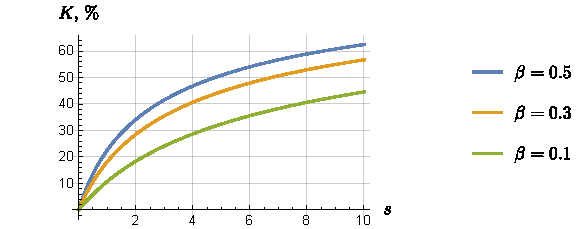
\includegraphics[width=0.5\textwidth]{"D:\\Kami\\git_folder\\notes_5sem\\rqc\\saturation_spectr_simulation\\K.pdf"}
    %\caption{}
    %\label{fig:}
\end{figure}


